\chapter{The $\CalS$-system}
    \label{sec:fine}
    \oldlabel{2}


\section{Overview}
    \label{sec:fine-overview}
    \oldlabel{2.1}



In this \chap, we define a decomposition of a $V$-cell. Let
$\op{VC}$ be the $V$-cell at the origin.  For any $t > 0$, let
$V(t)$ be the intersection of $\op{VC}$ with the ball $B(0,t)$ at
the origin of radius $t$. We write $\op{VC}$ as the disjoint union
of $V(t_0)$ and its complement $\delta$.

Assume that there is an upright quarter in the $Q$-system with
diagonal $\{0,v\}$. As usual, we call $\{0,v\}$ an {\it upright diagonal}.
We will define $\delta(v)\subset\delta$. It will be a subset of a
set of the form $C(D_v)\cap\delta$ for some subset $D_v$ of the
unit sphere.  The sets $D_v$ will be defined so as not to overlap
one another for distinct $v$. Then the sets $\delta(v)$ do not
overlap one another either. We will give an explicit formula for
the volume of $\delta(v)$.

We will define a set $\CalS$ of simplices, each having a vertex at
the origin. (The letter `$\CalS$' is for simplex.)
The vertices of the simplices will be vertices of the
packing, and their edges will have length at most $2\sqrt{2}$. The
sets $C(S)$, for distinct $S\in\CalS$, will not overlap. Over a
simplex $S\in\CalS$, the $V$-cell will be truncated at a radius
$t_S\ge t_0$. After defining the constants $t_S$, we will set
    $$V_S(t_S) = C(S) \cap V(t_S) =C(S)\cap B(t_S)\cap \op{VC}(0).$$
That is, $V_S(t_S)$ is the part of the $V$-cell at the origin,
contained in the cone over $S$ and in the ball of radius $t_S$.
If
    $\op{VC}(0) \cap C(S)\subset B(t_S)\subset B(t'_S)$,
then
    $V_S(t_S)=V_S(t'_S)$.

Since $t_S\ge t_0$, the sets $V_S(t_S)$ and $\delta$ may overlap.
Nevertheless, we will show that $V_S(t_S)$ does not overlap any
$\delta(v)$.  Let $\tildeV(t_0)$ be the set of points in $V(t_0)$
that do not lie in $C(S)$, $S\in\CalS$.  We will derive an
explicit formula for the volume of $\tildeV(t_0)$.

In $\op{VC}(0)$, there are nonoverlapping sets
$$\delta(v),\quad   V_S(t_S),\quad \tildeV(t_0).$$
Let $\delta'$ be the complement in $\op{VC}(0)$ of the union of
these sets. These sets give a decomposition of $\op{VC}(0)$.
Corresponding to this decomposition is a formula for $\sigma(D)$
of the form
    $$
    \sigma(D) =
        \op{c-vor}(\tildeV(t_0))
        + \sum_{\CalS}\op{c-vor}(V_S(t_S))
        -\sum_v 4\doct\op{vol}(\delta(v))-4\doct\op{vol}(\delta').
    $$
Since $\op{vol}(\delta')\ge0$, we obtain an upper bound on
$\sigma(D)$ by dropping the rightmost term.



\section{The set $\delta(v)$}
    \label{sec:deltaP}
    \oldlabel{2.3}

Let $\{0,v\}$ be the diagonal of an upright quarter in $\CalQ_0$. We
define $\delta(v)\subset C(D_v)\cap \delta$ for an appropriate
subset $D_v$ of the unit sphere.

\begin{definition}\label{def:eta0}
Set $\eta_0(h)=\eta(2h,2,2t_0)$.
\index{zzeta@$\eta_0$}
\end{definition}

If $h\le\sqrt2$, then $\eta_0(h)\le \eta_0(\sqrt2) <
1.453$.\index{ZZZZ1.453@1.453}

Let $D_0$ be the spherical cap on the unit sphere, centered along
$\{0,v\}$ and having arcradius $\theta$, where
    $\cos\theta = |v|/(2\eta_0(|v|/2))$.


The area of $D_0$ is
    $2\pi(1-\cos\theta)$.
Let $v_1,\ldots,v_k$ be the anchors around $\{0,v\}$ indexed
cyclically. The radial projections of the edges $\{v,v_i\}$
(extended as necessary) slice the spherical cap into $k$ wedges
$W_i$, between
    $\{v,v_i\}$ and $\{v,v_j\}$,
where $j\equiv i+1\mod k$, so that
    $D_0 =\cup W_i$.

\begin{definition}\label{def:wedge}
Let $\CalW$ be the set of wedges $W=W_i$  such that either
\begin{enumerate}
    \item $W$ occupies more than half the spherical cap (so that
    its area is at least $\pi(1-\cos\theta)$), or
    \item
 $|v_i-v_j|\ge 2.77$,
    $\rad(0,v,v_i,v_j)\ge\eta_0(|v|/2)$, and the
    circumradius of $\{0,v_i,v_j\}$ or $\{v,v_i,v_j\}$ is
    $\ge\sqrt2$.
    \label{enum:wedge2}
\end{enumerate}
\index{wedge}
\index{W@$\CalW$}
\end{definition}

Fix $i,j$, with $j\equiv i+1\mod k$. If $W = W_i$ is a wedge in
$\CalW$, let $\{0,v_i,v\}^\perp$ be the plane through the origin and
the circumcenter of $\{0,v_i,v\}$, perpendicular to $\{0,v_i,v\}$.
Skip the following step if the circumradius of $\{0,v_i,v\}$ is
greater than $\eta_0(|v|/2)$, but if the circumradius is at most
this bound, let $c_i$ be the intersection of $\{0,v_i,v\}^\perp$
with the circular boundary of $W$.  Extend $W$ by adding to $W$
the spherical triangle with vertices the radial projections of
$v$, $v_i$, and $c_i$.  Similarly, extend $W$ with the triangle
from $\{v,v_j,c_j\}$, if the circumradius of $\{0,v_j,v\}$ permits.
(An example of this is illustrated in
Fig.~\ref{fig:anchor-quarter}.) Let $W^e$ be extension of the
wedge obtained by adding these two spherical triangles.
\index{W@$W^e$}

\begin{figure}[htb]
  \centering
  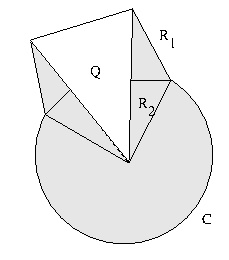
\includegraphics{PS/diag46.ps}
  \caption{An example of a set $W^e$ (shaded region).}
  \label{fig:anchor-quarter}
\end{figure}

We will define
    $\delta(v,W^e)\subset C(W^e)\cap \delta$.
Then $\delta(v)$ is defined as the union of $\delta(v,W^e)$, for
$W\in\CalW$. Let
    $$E_w = \{x : 2 x\cdot w \le w\cdot w\},$$
for $w = v,v_i,v_j$. These are half-spaces bounding the Voronoi
cell. Set $E_\ell = E_{v_\ell}$.

If (2) holds, we let $c$ be the radial projection of the
circumradius of $\{0,v_i,v_j,v\}$ to the unit sphere.  The arclength
from $c$ to the radial projection of $v$ is $\theta'$, where
$$\cos\theta' = |v|/(2\rad)<|v|/(2\eta_0) = \cos\theta.$$
We conclude that $\theta'>\theta$ and $c$ does not lie in $D_0$.

\begin{definition} \label{def:delta-e}
In both cases (1) and (2), set
    $$
    \begin{array}{lll}
    \Delta(v,W^e) &= (E_v\cap E_i\cap E_j \cap C(W^e))\\
    \delta(v,W^e) &= \Delta(v,W^e)\setminus B(t_0).
    \end{array}
    $$
\index{zzdelta@$\delta(v,W^e)$}
\index{zzDelta@$\Delta(v,W^e)$}
\end{definition}

\begin{remark}
There are some degenerate cases in this construction depending on
the number of anchors.  If there is no anchor, then
$\Delta(v,W^e)$ is to be defined simply as $(E_v \cap C(W^e))$.
If there is one anchor $v_i$, then
    $$
    \Delta(v,W^e) = (E_v\cap E_i\cap C(W^e)).
    $$
\end{remark}

\begin{remark}
The following remark applies when the points $c_i$ and $c_j$ have
been constructed, and is irrelevant when that step was skipped in
the construction described above. Observe that
    $$E_v\cap E_i\cap E_j \cap C(W^e)$$
is the union of four Rogers simplices
    $$
    R(|w|/2,\eta(0,v,v_\ell),\eta_0(|v|/2)),
    \quad w = v,v_\ell,\quad
    \ell = i,j
    $$
and a conic wedge over $W$ between $c_i$ and $c_j$. (The
inequality $\theta'>\theta$ implies that the Rogers simplices do
not overlap.)
\end{remark}

In general, we break $\Delta(v,W^e)$ into an inner part
$\Delta^-(v,W^e)$ (the part outside the Rogers simplices together
with (as many as) two Rogers simplices along $(0,v)$), and the
Rogers simplices $R_w$, for $w=v_i,v_j$.  We take $R_w$ to be the
empty set, when there is no anchor $w$ with
$\eta(0,v,w)<\eta_0(|v|/2)$.
\index{zzDelta@$\Delta^-(v,W^e)$}
\index{R@$R_w$}



We present a series of lemmas that explore the geometry of the sets
$\Delta(v,W^e)$.  In the next few lemmas we make use of a function
$\epsilon$, which is defined as follows.

\begin{definition}
If $\Lambda$ is a set of vertices containing $v$,
 let
$\epsilon_v(\Lambda,x)\in \Lambda$ be given as the vertex $w\in
\Lambda\setminus\{v\}$ such that the ray from $v$ through $x$
intersects the perpendicular bisecting plane of $\{v,w\}$ before
that of any other $w'\in \Lambda\setminus\{v\}$. If the ray from
$v$ through $x$ does not intersect any of the planes, then we set
$\epsilon$ to the default value $v$. In cases of ties, resolve the
tie in any consistent manner. If $x\in \Omega(0)$ (the Voronoi
cell at the origin), then $x$ lies in the cone over the face
attached to the vertex $\epsilon_0(\Lambda,x)\in \Lambda$.
\index{zzepsilon@$\epsilon_v(\Lambda,x)$}

We define a function $\epsilon'$ in a similar fashion. Assume
$\epsilon_v(\Lambda,x)=w$, where the ray from $v$ to $x$
intersects the perpendicular bisector to $\{v,w\}$ at $x'$. Set
  $$
  \epsilon'_v(\Lambda,x)=\epsilon_{w/2}(\Lambda\setminus\{w\},x').
  $$
\index{zzepsilon'@$\epsilon'_v(\Lambda,x)$} That is, move along
the face of the Voronoi cell from $x$ until another face is
encountered.  Let the corresponding vertex be the value of
$\epsilon'$.  If $x\in \Omega(0)$ in the cone over the face
attached to the vertex $w$, and if $w/2$ lies on that face, then
$x'$ lies in the sector of the face formed by the cone at $w/2$
generated by the edge of the Voronoi cell between the faces
associated to $w$ and $\epsilon'_0(\Lambda,x)$.
\end{definition}

\begin{lemma}\label{lemma:prev}
Let $S=\{0,v,w,u\}$ be a simplex.  Assume that $\{0,v\}$ is an
upright diagonal of a quarter in the $Q$-system, that $w$ and $v$
are anchors of $\{0,v\}$, and that $\rad(S)< \eta_0(|v|/2)$.
Assume there is a wedge $W$ of $\CalW$ along the face $\{0,v,w\}$
(on the same side of the face as $u$).  Let $R_w$ be the Rogers
simplex $R(|w|/2,\eta(0,v,w),\eta_0(|v|/2))$ along the face
$\{0,w,v\}$ along the edge of $\{0,w\}$ on the same side of the
face as $u$.  Then
\begin{enumerate}
\item There exists an anchor $w'$ between $u$ and $w$ with
    $|w-w'|\le 2t_0$, and $|w'-w|\ge2.77$.
\item $\{0,v,u,w'\}$ is an upright quarter in the $Q$-system and
its face $\{0,v,w'\}$ is a barrier.
 \item  The barrier $\{0,v,w'\}$ obstructs every point of $R_w$
 from $u$.
\end{enumerate}
\end{lemma}


\begin{proof}
Since $\rad(S) <\eta_0(|v|/2)$ is contrary to the conditions
defining wedges, the wedge must run from the face $\{0,v,w\}$ to a
face $\{0,v,w'\}$, where $w'$ is an anchor between $w$ and $u$. By
the hypotheses defining wedges $W\in\CalW$, we have that the
length of $\{u,w'\}$ is at least $2.77$. For the same reason, the
circumradius of $\{0,v,w,w'\}$ is at least $\eta_0(|v|/2)$.

%We reach a similar contradiction if $\{0,w'\}$ passes through
%$\{0,u\}$.  These facts imply that $w$ lies in the convex hull of
%$\{0,v,u,w\}$.

We claim that $R_w$ lies in the convex hull of $S=\{0,v,w,w'\}$.
Since $|w-w'|\ge 2.77$, we see that the orientation of each face
of $\{0,v,w,w'\}$ is positive.  Since $\op{rad}(S)\ge \eta_0$, we
have
  $$
  R_w \subset R(|w|/2,\eta(0,v,w),\op{rad}(S)) \subset S.
  $$
Thus it is enough to show that each point of the convex hull of
$S$ is obstructed.

For this, it is enough to show that the extreme point $w$ is
obstructed from $u$ by the barrier $\{0,v,w'\}$.  In other words,
we show that the edge $\{w,v\}$ passes through $\{0,v,w'\}$.  For
this we show that no other geometrical configuration of points is
possible.

$w'$ is not in the convex hull of $\{0,v,w,u\}$ by
Lemma~\ref{lemma:v-interior-alt}. The vertex $w'$ is not enclosed
over $\{0,v,w,u\}$ because
    $$
    \CalE(S(2,2,2t_0,2t_0,2t_0,2(1.453),2,2,2)> 2t_0.
    $$
(The constant $1.453$ is from Definition~\ref{def:eta0}.)  The
edge $\{v,w'\}$ does not pass through $\{0,w,u\}$, for otherwise
we would reach a contradiction
    $$
    2\eta_0(|v|/2) > 2\rad(S) \ge |u-w| \ge
    \CalE(S(2,2,2,\sqrt8,2,2),2,2,2.77) \ge 2(1.453) \ge
    2\eta_0(|v|/2).
    $$
We conclude that $\{u,w\}$ passes through $\{0,v,w'\}$.
\end{proof}

\begin{lemma}\label{lemma:delta-tri}
Let $F=\{0,u_1,u_2\}$ be a quasi-regular triangle.  Let $\{0,v\}$ be
the diagonal of an upright quarter in the $Q$-system. The set
$\Delta(v,W^e)$ does not overlap the cone at $0$ over the triangle
$F$.
\end{lemma}

\begin{proof}
We prove the lemma for the subsets $\Delta^-(v,W^e)$ and $R_w$ in
two separate cases, beginning with $\Delta^-(v,W^e)$.  Let $S$ be the simplex
$\{0,u_1,u_2,v\}$.

Assume that the orientation of $S$ along $F$ is negative.  The
simplex $S$ is an upright quarter, so that $u_1$ and $u_2$ are
anchors of $v$. This is contrary to the construction of the wedges
$W$ in $\CalW$. Thus, the orientation of $F$ must be positive.

Assume that $\rad(S)< \eta_0(|v|/2)$.  Then again, $u_1$ and $u_2$
are anchors.  It follows that $S$ is an upright quarter.  As in
the previous paragraph, this is contrary to construction.  Thus,
$\rad(S)\ge \eta_0(|v|/2)$.



We now have that the orientation of $F$ is positive and that $\rad(S)\ge \eta_0(|v|/2)$.
These two facts allow us to separate $\Delta^-(v,W^e)$ from $\{0,u_1,u_2,v\}$ as follows.
Each interior point $x$ of $\Delta^-(v,W^e)$ has
$$\epsilon_0( \{ 0,u_1,u_2,v \} ,x) = v.$$
Let $F_0$ be the set of  points in the intersection of $\Omega(0)$
with the convex hull of $F$.  Each point $y$ in $F_0$ has
$$\epsilon_0( \{ 0,u_1,u_2,v \} ,y) \in \{u_1,u_2\}.$$
Since $\epsilon_0$ takes distinct values on these two sets, they
are disjoint.

Next consider the subset $R_w$, in the case that $w\in\{u_1,u_2\}$.  To be definite,
assume that $w=u_1$.  The same argument as above establishes that
the orientation of $F$ is positive and that $\rad(S) \ge \eta_0(|v|/2)$.
Each interior point $x$ of $R_w$ has
$$\epsilon'_0( \{ 0,u_1,u_2,v \} ,x) = v$$
But each point $y$ in $F_0$ has
$$\epsilon'_0( \{ 0,u_1,u_2,v \} ,y) \in \{u_1,u_2\}.$$
This proves this case.


Until the end of the proof, we may assume that
$w\not\in\{u_1,u_2\}$.  If the value of
$\epsilon_0(\{0,u_1,u_2,w\},\cdot)$ is $w$ on interior points of
$R_w$ and in $\{u_1,u_2\}$ on $F_0$, then we have separated the
sets.  Assume to the contrary, that $\epsilon$ takes value $w$ at
a point $x$ of $F_0$.  Let $S''=\{0,u_1,u_2,w\}$.  This assumption
implies that the orientation of $S''$ is negative along $F$.  This
in turn implies that $S''$ is a quasi-regular tetrahedron.  The
vertex $v$ is not enclosed over $S''$, because the simplices in
the $Q$-system do not overlap.  For similar reasons, the face
$\{0,v,w\}$ does not overlap the simplex $S''$.  By the previous
case (when $w\in\{u_1,u_2\}$), the interior of $R_w$ does not
intersect the faces of the quasi-regular tetrahedron $S''$ along
the edge $\{0,w\}$.  These facts imply that The interior of $R_w$
is disjoint from $S''$.  In particular, it does not meet the cone
at $0$ over the triangle $F$.

Assume finally that $\epsilon$ takes value $u_1$ or $u_2$ at an
interior point $y$ of  $R_w$. (Say $u_1$.)     Let
$S'=\{0,v,w,u_1\}$. Assume that $R_w$ lies on the same side of
$\{0,v,w\}$ as $u_1$.  If $\rad(S') < \eta_0(|v|/2)$, then each
point of $R_w$ is obstructed from $u_1$ (by
Lemma~\ref{lemma:prev}).  But no point of $F_0$ is obstructed from
$u_1$.  Thus, $R_w$ and $F_0$ are disjoint in this case.  Assume
that $\rad(S') \ge \eta_0(|v|/2)$.  If the orientation of
$\{0,v,w\}$ in $S'$ is negative, then $S'$ is a quarter and the
result follows.  Assume that the orientation is positive.  Now
$\epsilon_0(S',x) = w$ for $x\in R_w$, contrary to assumption.

We may now assume that $R_w$ lies outside the simplex $S'$ on the
opposite side of the face $\{0,v,w\}$. This case is dismissed by
Lemma~\ref{lemma:back}, which guarantees that the interior of
$R_w$ with $\epsilon=u_1$ are obstructed from $u_1$ by
$\{0,v,w\}$.  However, none of the points of $F_0$ with
$\epsilon=u_1$ are obstructed from $u_1$.
\end{proof}

\begin{corollary}
Each $\Delta(v,W^e)$ lies entirely in the cone over the standard
region that contains $\{0,v\}$.
\end{corollary}

\begin{proof}
The cone over a standard region is bounded by the cones  over the
quasi-regular triangles.
\end{proof}




\begin{lemma}\label{lemma:delta-flat}
Let $F=\{0,u_1,u_2\}$ be a triangle.  Assume that $|u_1|\le 2t_0$,
$|u_2|\le 2t_0$, and $2t_0\le|u_1-u_2|\le\sqrt8$.  Let $\{0,v\}$
be the diagonal of an upright quarter in the $Q$-system.  Assume
that if $u_1$ and $u_2$ are both anchors of $v$, then they are
consecutive anchors around $v$. Under these conditions, the set
$\Delta(v,W^e)$ does not overlap the cone at $0$ over the triangle
$F$.
\end{lemma}

\begin{proof} The proof is similar to that of
Lemma~\ref{lemma:delta-tri}.  We prove the lemma for the subsets
$\Delta^-(v,W^e)$ and $R_w$ in two separate cases, beginning with
$\Delta^-(v,W^e)$.  Let $S$ be the simplex $\{0,u_1,u_2,v\}$. The
orientation of $S$ along $F$ is positive.

Assume that $\rad(S)< \eta_0(|v|/2)$.  Then $u_1$ and $u_2$ are
anchors.  By the hypotheses of the lemma, they are consecutive
anchors.  By the rules defining $\Delta^-(v,W^e)$, there is no
wedge $W^e$ between $u_1$ and $u_2$.  Thus, the result follows in
this case.


We now have that the orientation of $F$ is positive and that
$\rad(S) \ge \eta_0(|v|/2)$. These two facts allow us to separate
$\Delta^-(v,W^e)$ from the cone over $\{0,u_1,u_2,v\}$ as follows.
Each interior point $x$ of $\Delta^-(v,W^e)$ has
$$\epsilon_0( \{ 0,u_1,u_2,v \} ,x) = v.$$
Let $F_0$ be the intersection of $\Omega(0)$ with the convex hull
of $F$.  Each point $y$ in $F_0$  has
$$\epsilon_0( \{ 0,u_1,u_2,v \} ,y) \in \{u_1,u_2\}.$$

Next consider the subset $R_w$, in the case that
$w\in\{u_1,u_2\}$.  To be definite, assume that $w=u_1$.  The same
argument as above establishes that the orientation of $F$ is
positive and that $\rad(S) \ge \eta_0(|v|/2)$. Each interior point
$x$ of $R_w$ has
$$\epsilon'_0( \{ 0,u_1,u_2,v \} ,x) = v$$
But each point $y$ in $F_0$ has
$$\epsilon'_0( \{ 0,u_1,u_2,v \} ,y) \in \{u_1,u_2\}.$$
This proves this case.

Consider the subset $R_w$, in the case that $w\not\in\{u_1,u_2\}$.
As in the previous proof, if the value of
$\epsilon_0(\{0,u_1,u_2,w\},\cdot)$ is $w$ on interior points of
$R_w$ and in $\{u_1,u_2\}$ on $F_0$, then we have separated the
sets.  Assume first to the contrary, that $\epsilon_0$ takes value
$w$ at a point $x$ of $F_0$.  Let $S''=\{0,u_1,u_2,w\}$.  Our
assumption on $\epsilon_0$ implies that the orientation of $S''$
is negative along $F$, so that $S''$ is a flat quarter.  The
vertex $v$ cannot be enclosed over $S''$, for otherwise $w$,
$u_1$, and $u_2$ would all be anchors of $v$, which would mean
that there is no region $W\in\CalW$.  Similarly, the triangle
$\{0,v,w\}$ cannot overlap the triangle $\{0,u_1,u_2\}$, for
otherwise $w$, $u_1$, and $u_2$ would again be anchors, contrary
to the hypothesis that $u_1$ and $u_2$ are consecutive anchors.
Now we invoke Lemma~\ref{lemma:delta-tri}, to establish that $R_w$
does not intersect $S''$ and is therefore disjoint from $F_0$.

Assume finally, that $\epsilon_0$ takes value $u_1$ or $u_2$ at an
interior point $y$ of  $R_w$. (Say $u_1$.)   This case is
identical to the parallel case in the proof of
Lemma~\ref{lemma:delta-tri}.
\end{proof}

\begin{lemma}\label{lemma:delta-upright}
Let $F=\{0,u_1,u_2\}$ be a triangle.  Assume that $2t_0\le|u_1|\le
\sqrt8$, $2\le|u_2|\le 2t_0$, and $2\le|u_1-u_2|\le2t_0$.  Let
$\{0,v\}$ be the diagonal of an upright quarter in the $Q$-system.
Under these conditions, the set $\Delta(v,W^e)$ does not overlap
the cone at $0$ over the triangle $F$.
\end{lemma}

\begin{proof}
Let $S=\{0,u_1,u_2,v\}$.  The orientation of $S$ along
$\{0,u_1,u_2\}$ is positive.  The circumradius $\rad(S)$ is at
least $\eta_0(0,v,u_1)\ge\eta_0(|v|/2)$.

We now have that the orientation of $F$ is positive and that
$\rad(S) \ge\eta_0(|v|/2)$.  We can then argue as in the proof of
Lemmas~\ref{lemma:delta-tri} and \ref{lemma:delta-flat}, to get
the result for $\Delta^-(v,W^e)$ and $R_{w}$ (with $w=u_2$).

Consider the case $R_w$, with $w\ne u_2$.  As in these earlier
proofs, we may assume  that $\epsilon_0$ takes value $w$ at a
point $x$ of $F_0$ (or that $\epsilon_0$ takes value in
$\{u_1,u_2\}$ at a point $y$ of $R_w$).

In the case $\epsilon_0=w$ at $x\in F_0$, let
$S''=\{0,u_1,w,u_2\}$. We have that $\epsilon_0=w$ implies that
the orientation of $S''$ along $\{0,u_1,u_2\}$ is negative.  This
in turn implies that $S''$ is an upright quarter.  It is checked
without difficulty that $v$ is not enclosed over $S''$ and that
the face $\{0,w,v\}$ does not cross the face $\{0,u_1,u_2\}$.  It
follows from Lemma~\ref{lemma:delta-tri} and the already treated
cases of this lemma that $R_w$ cannot intersect $S''$.  Thus, it
does not intersect the face $\{0,u_1,u_2\}$ of $S''$.

Finally, assume that $\epsilon_0$ takes value in $\{u_1,u_2\}$ at
a point $y$ of $R_w$.  The orientation of the face $\{0,v,w\}$ is
positive in the simplex $\{0,v,w,u_1\}$ and the circumradius of
$\{0,v,w,u_1\}$ is greater than $\eta_0(|v|/2)$.  This implies
that $\epsilon_0$ does not take the value $u_1$.  Assume that
$\epsilon_0=u_2$.  This case is excluded in the same manner as the
parallel case in the earlier Lemmas~\ref{lemma:delta-tri} and
\ref{lemma:delta-flat}.
\end{proof}

\begin{lemma}
Let $\{0,v\}$ be an upright diagonal of a quarter in the
$Q$-system.   If $x$ lies in the interior of $\Delta(v,W^e)$,
then $x$ is unobstructed at $0$.
\end{lemma}

\begin{proof} For a contradiction, assume that $x$ is obstructed
at $0$ by barrier $T =\{u_1,u_2,u_3\}$.


The convex hull of $T$ can be partitioned into three sets $T(i)$
depending on which vertex of $T$ is closest to a given point in
the convex hull. (Ties can be resolved in any consistent manner.)
Let $y\in \Delta(v,W^e)$ be the point in the convex hull of $T$ on
the segment from $0$ to $x$.  Fix $i$ so that $y\in T(i)$. If
$v=u_i$, then each point $y$ of $T(i)$ is closer to $v$ than to
$0$.  But each point of $\Delta(v,W^e)$ is closer to $0$ than to
$v$.  So $x$ is not obstructed by $T$ at $0$.

We may now assume that $v\ne u_i$.

Partition $\ring{R}^3$ geometrically into three sets $V(u_i)$,
$V(0)$, $V(v)$ according to which of $\{u_i,0,v\}$ a point
$z\in\ring{R}^3$ is closest to.  (Again resolve ties in any
consistent manner.)

Assume further that $\max_j u_j \ge 2t_0$. This implies that $y\in
T(i) \subset V(v) \cup V(u_i)$.  On the other hand, we have by
construction that $y\in \Delta(v,W^e) \subset V(0)$.  (There are
two cases involved in this conclusion, depending on whether $u_i$
is an anchor of $\{0,v\}$.)  However, the sets $V(\cdot)$ are
disjoint; and we reach a contradiction.  Thus, under these
assumptions, $x$ is unobstructed at $0$.

Next assume that $\max_j u_j < 2t_0$.  Let $S=\{0,u_1,u_2,u_3\}$.
Since $T$ is a barrier, $S\in\CalQ_0$.  By assumption, $\{0,v\}$
is a diagonal of an upright quarter in $\CalQ_0$.  By the
nonoverlap of quarters in $\CalQ_0$, we see that $v$ is not
enclosed over $S$. The wedge $W^e$ on the unit sphere is
spherically star convex with respect to the center $v/|v|$.  Thus,
if $\Delta(v,W^e)$ intersects the convex hull of $T$ at $y$, then
$\Delta(v,W^e)$ intersects the cone over a face $\{0,u_1,u_2\}$ of
$S$ at $y'$. (We can take $y'/|y'|$ to lie on the cone generated
by the arc running from $v/|v|$ to $y/|y|$. This is impossible by
Lemmas~\ref{lemma:delta-tri} and \ref{lemma:delta-flat}.
\end{proof}

\begin{lemma}  Let $\{0,v\}$ be the upright diagonal of a quarter
in the $\CalQ_0$-system.  Then the interior of $\Delta(v,W^e)$ is
a subset of $\op{VC}(0)$.
\end{lemma}

\begin{proof}
We begin by showing that $\Delta^-(v,W^e)\subset\op{VC}(0)$.
Suppose to the contrary, that a point $x$ in the interior of
$\Delta^-$ lies in $\op{VC}(w)$, with $w\ne0$.  Then $x$ is closer
to $w$ than to  $0$.  Thus, $\eta(0,v,w)<\eta_0(|v|/2)$, and $w$
is an anchor of $\{0,v\}$.  The face $E_w$ in the construction
$\Delta^-(v,W^e)$ prevents this from happening.

Now consider a point $x$ of $R_w$, which we assume to lie in
$\op{VC}(u)$, with $u\ne0$.  To avoid a trivial case, we may
assume that $w\ne u$.

Assume that the orientation of $S=\{0,v,w,u\}$ is negative along
the face $\{0,v,w\}$.  Then $S$ must be an upright quarter.  By
the construction of wedges $W\in\CalW$, we have that $R_w$ must
lie on the opposite side of the plane $\{0,v,w\}$ from $u$ (for
there is no wedge between the anchors of an upright quarter).  The
result now follows from Lemma~\ref{lemma:back}.

If $\rad(S) <\eta_0(|v|/2)$, then $u$ and $w$ are anchors.  In
this case, the result follows from Lemma~\ref{lemma:prev}.

Finally if the orientation is positive and if $\rad(S)\ge
\eta(|v|/2)$, then a point of $R_w$ cannot be closer to $u$ than
to $0$.
\end{proof}


\section{Overlap}
    \label{sec:overlap}
    \oldlabel{2.4}


\begin{lemma}  The sets $\Delta(v,W^e)$ do not overlap one another.
\end{lemma}

\begin{proof}
This is clear for two sets around the same vertex $v$.  Consider
the sets $\Delta(u,W^e)$ and $\Delta(v,W^e)$ at $u$ and $v$.
%In general,
%this follows from the fact that the sets $W^e$ do not overlap on
%the unit sphere.  We use the faces of the $V$-cell to separate
%them. In the notation of Sections~\ref{sec:fine-overview} and
%\ref{sec:deltaP}, the part of the wedge $W$ between $c_i$ and
%$c_j$ lies under the face of the $V$-cell associated with $v$, the
%vertex used to construct $W$. Hence, these pieces do not overlap
%at different vertices. Similarly, two of the Rogers simplices lie
%under the face of the $V$-cell associated with $v$. The remaining
%two Rogers simplices lie under the faces of $V$-cells of two of
%the anchors of $v$. A vertex $v_i$ may be the anchor of more than
%one upright diagonal $(0,v)$ and $(0,v')$. Nevertheless, the
%corresponding Rogers simplices do not overlap because each Rogers
%simplex for $W^e$ at $v$ will lie under the triangular part of the
%face determined by $v_i/2$ and the edge of the $V$-face dual to
%the triangle $(0,v_i,v)$, and the Rogers simplex for $W^{\prime
%e}$ at $v'$ will lie under a corresponding triangular part of the
%face.  These triangles do not overlap, so the extended wedges
%cannot either.

To treat the points in $\Delta^-(u,W^e)$ and $\Delta^-(v,W^e)$, we
may contract $\{u,v\}$ until $|u-v|=2$.  By the constraints on the
edges of $\{0,u,v\}$, the circumcenter $c$ of this triangle lies
in the convex hull of the triangle.  We have $\eta(0,u,v)\ge
\eta_0(|v|/2)$ and $\eta(0,u,v)\ge\eta_0(|u|/2)$.  So the plane
through $\{0,c\}$ perpendicular to the plane $\{0,u,v\}$ separates
$\Delta^-(u,W^e)$ from $\Delta^-(v,W^e)$.

Next we separate points in $\Delta^-(u,W^e)$ from points of
$R_w^{(v)}$, where $w$ is an anchor of $v$ and $u\ne v$.  Let
$S=\{0,u,v,w\}$. The orientation of $S$ along $\{0,v,w\}$ is
positive.  The circumradius of $S$ satisfies
    $$
    \rad(S) \ge \eta(0,u,v)>\eta_0(|v|/2).
    $$
Thus, $\epsilon_0(S,\cdot)$ takes different values on
$\Delta^-(u,W^e)$ and $R_w^{(v)}$, so that the sets are disjoint.

Next we separate points of $R_w^{(v)}$ from $R_w^{(u)}$.  (Notice
that we assume that the anchor is the same for the two Rogers
simplices.) Let $S=\{0,u,v,w\}$.   As above, we have
    $$
    \rad(S) \ge \eta_0(|v|/2), \quad \eta_0(|w|/2).
    $$
The simplex $S$ has positive orientation along the faces
$\{0,u,w\}$ and $\{0,v,w\}$.  Let $c_u$ be the circumcenter of
$\{0,u,w\}$, let $c_v$ be the circumcenter of $\{0,v,w\}$, and let
$c$ be the circumcenter of $S$.  Then $R_w^{(v)}$ lies in the
convex hull of $\{0,w,c_v,c\}$, but $R_w^{(u)}$ lies in the convex
hull of $\{0,w,c_u,c\}$.  Thus, the sets are disjoint.

Finally, we separate points of $R_w^{(u)}$ from points of
$R_{w'}^{(v)}$, where $w\ne w'$ and $u\ne v$.  If the function
$\epsilon_0(\{0,w,w'\},\cdot)$ separates the sets, we are done.
Otherwise, we may assume say that $\epsilon_0(\{0,w,w'\},x) = w'$
from some $x\in R_w^{(u)}$.  Let $S=\{0,u,w,w'\}$.

If $w'$ is not an anchor of $u$, then $\rad(S) \ge\eta_0(|u|/2)$
and the orientation of $S$ along $\{0,w,u\}$ is positive.  In this
case, we have $\epsilon_0 = w$ on $R_w^{(u)}$, which is contrary
to assumption. Thus, we may assume that $w'$ is an anchor of $u$.

If the orientation of $\{0,u,w,w'\}$ is negative along
$\{0,w,u\}$, then $\{0,u,w,w'\}$ is a quarter, contrary to the
existence of $W\in \CalW$.  So the orientation is positive.  If
$\rad(\{0,u,w,w'\}) < \eta_0(|u|/2)$, then Lemma~\ref{lemma:prev}
implies that each point of $R_w$ is obstructed from $w'$.  But no
point of $R_{w'}^{(v)}$ is obstructed from $w$. (In fact, a
barrier that crosses $\Delta(v,W^e)$ is inconsistent with the
Lemmas~\ref{lemma:delta-tri}, \ref{lemma:delta-flat},
\ref{lemma:delta-upright}.) So $\rad(\{0,u,w,w'\}) \ge
\eta_0(|u|/2)$.  This is contrary to $\epsilon_0(\{0,w,w'\},x) =
w'$ from some $x\in R_w^{(u)}$.
\end{proof}

%Suppose that the faces of the $V$-cell dual to two vertices $v_1$
%and $v_2$(of height at most $2\sqrt{2}$) share an edge.  On the
%face dual to $v_1$, we take the triangle formed by $v_1/2$ and the
%common edge, and call it the $(v_1,v_2)$-triangle. (Since
%$|v_1|\le2\sqrt{2}$, $v_1/2$ lies on the face dual to $v_1$.) The
%proof shows that the set $\delta(v)$ lies under the face dual to
%$v$ or under the $(v_i,v)$-triangles of anchors $v_i$ of $v$.

\section{The $\CalS$-system defined}
    \oldlabel{2.5}

We consider three types of simplices $A$, $B$, $C$.  Each type has
its vertices at vertices of the packing.  The edge lengths of
these simplices are at most $2\sqrt{2}$.

$A$.  This family consists of simplices $S(y_1,\ldots,y_6)$ whose
edge lengths satisfy
    $$
    y_1,y_2,y_3\in[2,2t_0],\quad
    y_4,y_5\in[2t_0,2.77],
    \quad
    y_6\in[2,2t_0],\quad \text{and }
    \eta(y_4,y_5,y_6)<\sqrt{2}.
    $$
(These conditions imply $y_4,y_5<2.697$, because
$\eta(2.697,2t_0,2)>\sqrt2$.)

$\SB$.  This family consists of certain flat quarters that are
part of an isolated pair of flat quarters. It consists of those
satisfying $y_2,y_3\le 2.23$, $y_4\in[2t_0,2\sqrt{2}]$.

$\SC$.  This family consists of certain simplices
$S(y_1,\ldots,y_6)$ with edge lengths satisfying
    $y_1,y_4\in[2t_0,2\sqrt{2}]$, $y_2,y_3,y_5,y_6\in[2,2t_0]$.
We impose the condition that the first edge is the diagonal of
some upright quarter in the $Q$-system, and that the upper
endpoints of the second and third edges (that is, the second and
third vertices of the simplex) are consecutive anchors of this
diagonal. We also assume that $y_4< 2.77$, or that both face
circumradii of $S$ along the fourth edge are less than $\sqrt{2}$.

\begin{lemma}
    \label{lemma:2.77}
If a vertex $w$ is enclosed over a simplex $S$ of type $A$, $\SB$,
or $\SC$, then its height is greater than $2.77$.  Also, $\{0,w\}$
is not the diagonal of an upright quarter in the $Q$-system.
\end{lemma}

\begin{proof}
In case $A$, $\eta(y_4,y_5,y_6)<\sqrt{2}$, so an enclosed vertex
must have height greater than $2\sqrt{2}$.  It is too long to be
the diagonal of a quarter.

In case $\SB$, we use the fact that the isolated quarter does not
overlap any quarter in the $Q$-system.  We recall that a function
$\CalE$, defined in Section~\ref{sec:decomposition}, measures the
distance between opposing vertices in a pair of simplices sharing
a face. An enclosed vertex has length at least
    $$\CalE(S(2,2,2,2\sqrt{2},2t_0,2t_0),2t_0,2,2)>2.77.$$
By the symmetry of isolated quarters, this means that the diagonal
of a flat quarter must also be at least $2.77$.

In case $\SC$, the same calculation gives that the enclosed vertex
$w$ has height at least $2.77$.  Let the simplex $S$ be given by
$\{0,v,v_1,v_2\}$, where $\{0,v\}$ is the upright diagonal. By
Lemma~\ref{lemma:pass-anchor}, $v_1$ and $v_2$ are anchors of
$\{0,w\}$. The edge between $w$ and its anchor cannot cross
$\{v,v_i\}$ by Lemma~\ref{lemma:2t0-doesnt-pass-through}. (Recall
that two sets are said to {\it cross\/} if their radial
projections overlap.) The distance between $w$ and $v$ is at most
$2t_0$ by Lemma~\ref{lemma:double-face}. If $\{0,w\}$ is the
diagonal of an upright quarter, the quarter takes the form
$\{0,w,v_1,v_3\}$, or $\{0,w,v_2,v_3\}$ for some $v_3$, by
Lemma~\ref{lemma:double-face}. If both of these are quarters, then
the diagonal $\{v_1,v_2\}$ has four anchors $v$, $w$, $0$, and
$v_3$. The selection rules for the $Q$-system place the quarters
around this diagonal in the $Q$-system. So neither $\{0,w,v_1,v_3\}$
nor $\{0,w,v_2,v_3\}$ is in the $Q$-system. Suppose that
$\{0,w,v_1,v_3\}$ is a quarter, but that $\{0,w,v_2,v_3\}$ is not.
Then $\{0,w,v_1,v_3\}$ forms an isolated pair with $\{v_1,v_2,v,w\}$.
In either case, the quarters along $\{0,w\}$ are not in the
$Q$-system.
\end{proof}

\begin{remark}  The proof of this lemma does not make use of all the hypotheses
on $\SC$.  The conclusion holds for any simplex
$S(y_1,\ldots,y_6)$, with $y_1,y_4\in[2t_0,2\sqrt{2}]$,
$y_2,y_3,y_5,y_6\in[2,2t_0]$.
\end{remark}

\section{Disjointness}
    \oldlabel{2.6}

Let $S=\{0,v_1,v_2,v_3\}$ be a simplex of type $A$, $\SB$, or
$\SC$. An edge $\{v_4,v_5\}$ of length at most $2\sqrt{2}$ such
that $|v_4|,|v_5|\le 2t_0$ cannot cross two of the edges
$\{v_i,v_j\}$ of $S$.  In fact, it cannot cross any edge $\{v_i,v_j\}$
with $|v_i|,|v_j|\le 2t_0$ by Lemma~\ref{lemma:skew-quad}.  The
only possibility is that the edge $\{v_4,v_5\}$ crosses the two
edges with endpoint $v_1$, with $|v_1|\ge2t_0$ in case $\SC$.  But
this too is impossible by Lemma~\ref{lemma:double-face}.

Similar arguments show that the same conclusion holds for an edge
$\{v_4,v_5\}$ of length at most $2t_0$ such that $|v_4|\le2t_0$,
$v_5\le2\sqrt{2}$.  The only additional fact that is needed is
that $\{v_4,v_5\}$ cannot cross the edge between the vertex $v$ of
an upright diagonal $\{0,v\}$ and an anchor
(Lemma~\ref{lemma:2t0-doesnt-pass-through}).





\begin{lemma}
    \label{lemma:no-overlap}
    Consider two simplices $S$, $S'$, each of  type $A$, $\SB$, $\SC$,
or a quarter in the $Q$-system.
    Assume that $S$ and $S'$ do not lie
    in the cone over a quadrilateral region.  Then
    $S$ and $S'$ do not overlap.
\end{lemma}

\begin{proof}
By hypothesis, the standard region is not a quadrilateral, and we
thus exclude the case of conflicting diagonals in a quad cluster.
We claim that no vertex $w$ of $S$ is enclosed over $S'$.
Otherwise, $w$ must have height at least $2t_0$, so that $\{0,w\}$
is the diagonal of an upright in the $Q$-system, and this is
contrary to Lemma~\ref{lemma:2.77}. Similarly, no vertex of $S'$
is enclosed over $S$.

Let $\{v_1,v_2\}$ be an edge of $S$ crossing an edge $\{v_3,v_4\}$ of
$S'$. By the preceding remarks, neither of these edges can cross
two edges of the other simplex. The endpoints of the edges are not
enclosed over the other simplex. This means that one endpoint of
each edge $\{v_1,v_2\}$ and $\{v_3,v_4\}$ is a vertex of the other
simplex.  This forces $S$ and $S'$ to have three vertices in
common, say $0$, $v_2$, and $v_3$.  We have $S=\{0,v_1,v_3,v_2\}$
and $S'=\{0,v_3,v_2,v_4\}$. If
    $|v_2|\in[2t_0,2\sqrt{2}]$,
then we see that the anchors $v_3$, $v_4$ of $\{0,v_2\}$ are not
consecutive.  This is impossible for simplices of type $\SC$ and
upright quarters.  Thus, $v_2$ and $v_3$ have height at most
$2t_0$.  We conclude, without loss of generality, that
    $|v_4|\in[2t_0,2\sqrt{2}]$
and $|v_1-v_2|\ge 2t_0$.

The heights of the vertices of $S$ are at most $2t_0$, so it has
type $A$ or $\SB$, or it is a flat quarter in the $Q$-system. If
$S'$ is an upright quarter in the $Q$-system, then it does not
overlap an isolated quarter or a flat quarter in the $Q$-system,
so $S$ has type $\SA$. This imposes the contradictory constraints
on $\SA$
    $$
    2.77\ge |v_1-v_2|\ge\CalE(S(2t_0,2,2,2\sqrt{2},2t_0,2t_0),2,2,2)>2.77.
    $$
Thus $S'$ has type $\SC$.  This forces $S$ to have type $\SA$.  We
reach the same contradiction  $2.77\ge \CalE>2.77$.
\end{proof}

\section{Separation of simplices of type $\SA$}
    \label{sec:separation}
    \oldlabel{2.7}

Let $V_S = \op{VC}(0)\cap C(S)$, for a simplex $S$ of type $\SA$,
$\SB$, or $\SC$. We truncate $V_S$ to $V_S(t_S)$ by intersecting
$V_S$ with a ball of radius $t_S$.  The parameters $t_S$ depend on
$S$.

If $S$ has type $\SA$, we use $t_S=+\infty$ (no truncation).  If
$v$ is enclosed over $S=\{0,v_1,v_2,v_3\}$, then since
$\eta(v_1,v_2,v_3)<\sqrt{2}$, the face $\{v_1,v_2,v_3\}$ has
positive orientation for $S$ and $\{v,v_1,v_2,v_3\}$. This implies
that the $V$-cells at $v$ and $0$ do not intersect, and there is
no need to truncate.  If a simplex adjacent to $S$ has negative
orientation along a face shared with $\SA$, then it must be a
quarter $Q=\{0,v_4,v_1,v_2\}$ (Lemma
\ref{lemma:at-most-one-negative}) or quasi-regular tetrahedron. It
cannot be an isolated quarter because of the edge length
constraint $2.77$ on simplices of type $\SA$. If it is in the
$Q$-system, the face between $S$ and the adjacent simplex is a
barrier, and it does not interfere with the $V$-cell over $S$.
Assume that it is not in the $Q$-system. There must be a
conflicting diagonal $\{0,w\}$, where $w$ is enclosed over $Q$. ($w$
cannot be enclosed over $S$ by results of
Lemma~\ref{lemma:no-overlap}.) This shields the $V$-cell at $v_4$
from $C(S)$ by the two barriers $\{0,w,v_1\}$ and $\{0,w,v_2\}$ of
quarters in the $Q$-system.

This shows that nothing external to a simplex of type $\SA$
affects the shape of $V_S(t_S)$ (that is, $\op{VC}(0)\cap C(S)$
consists of points of $S$ that are closer to $0$ than to the other
vertices of $S$).  Thus,  $V_S(t_S)$ can be computed from $S$
alone. Similarly, $V_S(t_S)$ does not influence the external
geometry, since all faces have positive orientation.

We also remark that $V_S(t_S)$ does not overlap any of the sets
$\Delta(v,W^e)$.  This is evident from
Lemmas~\ref{lemma:delta-tri} and \ref{lemma:delta-flat}.

%because the two types of sets lie under the faces of $V$-cells
%associated with different vertices of the packing. A set
%$\delta(v)$ lies under the face of the $V$-cell dual to $v$ or
%under the $(w,v)$-triangles of anchors $w$ of $V$. But $V_S(t_S)$
%lies under the $(v_i,v_j)$-triangles, for the edges $(v_i,v_j)$ of
%$S$.  (See Section~\ref{sec:overlap}.)

Our justification that $V_S(t_S)$ can be treated as an
independently scored entity is now complete.

\section{Separation of simplices of type $\SB$}
    \oldlabel{2.8}

If $S(y_1,\ldots,y_6)$ has type $\SB$, we label vertices so that
the diagonal is the fourth edge, with length $y_4$. We set
$t_S=1.385$. The calculation of $\CalE$ in Lemma~\ref{lemma:2.77}
shows that any enclosed vertex over $S$ has height at least
$2.77=2t_S$.

Vertices outside $C(S)$ cannot affect the shape of $V_S(t_S)$.  In
fact, such a vertex $v'$ would have to form a quarter or
quasi-regular tetrahedron with a face of $S$.  The $V$-cell at
$v'$ cannot meet $C(S)$ unless it is a quarter that is not in the
$Q$-system. But by definition, an isolated quarter is not adjacent
(along a face along the diagonal) to any other quarters.

To separate the scoring of $V_S(t_S)$ from the rest of the
standard cluster, we also show that the terms of
Formula~\ref{eqn:3.5}  for $V_S(t_S)$ are represented
geometrically by solids that lie in the cone $C(S)$. This is more
than a formality because $S$ can have negative orientation along
the face $F$ formed by the origin and the diagonal (the fourth
edge).

\begin{definition}
Let
    $\beta_\psi(\theta)\in[0,\pi/2]$
be defined by the equations
    $$
        \cos^2\beta_\psi = (\cos^2\psi-\cos^2\theta)/(1-\cos^2\theta),
        \hbox{ for }\psi\le\theta,
    $$
Let $p$ and $q$ be points on the unit sphere separated by
arclength $\theta$. If we place a spherical cap of arcradius
$\psi$ on the unit sphere centered at $p$, then
$\beta_\psi(theta)$ is the angle at $q$ between the arc $(q,p)$
and the tangent to the cap which passes through $q$.
\end{definition}

Let $S=\{0,v_1,v_2,v_3\}$, where $v_i$ is the endpoint of the $i$th
edge. We establish that the solids representing the conic and
Rogers terms of Formula~\ref{eqn:3.5} lie over $C(S)$ by
showing\footnote{\calc{193836552}} that
    $\beta_\psi(\arc(y_1,y_3,y_5)) < \dih_3(S(y_1,\ldots,y_6))$,
where $\dih_3$ is the dihedral angle along the third edge. We use
$\cos\psi = y_1/2.77$ and assume $y_2,y_3\in[2,2.23]$.

The reasons given in Section~\ref{sec:separation} for the
disjointness of $\delta(v)$ and $V_S(t_S)$ apply to simplices of
type $\SB$ as well. This completes the justification that
$V_S(t_S)$ is an object that can be treated in separation from the
rest of the local $V$-cell.

\section{Separation of simplices of type $\SC$}
    \oldlabel{2.9}

If $S(y_1,\ldots,y_6)$ is of type $\SC$, we label vertices so that
the upright diagonal is the first edge.  We use $t_S =+\infty$ (no
truncation).   Each face of $S$ has positive orientation by
Lemma~\ref{lemma:at-most-one-negative}. So $V_S(t_S)\subset S$.

Vertices outside $S$ cannot affect the shape of $V_S(t_S)$.  Any
vertex $v'$ would have to form a quarter along a face of $S$.  If
the shared face lies along the first edge, it is a quarter $Q$ in
the $Q$-system, because one and hence all quarters along this edge
are in the $Q$-system.  The faces of this quarter are then
barriers. If the shared face lies along the fourth edge, then its
length is at most $2.77$, so that the quarter cannot be part of an
isolated pair. If it is not in the $Q$-system, there must be a
conflicting diagonal. The two faces along this conflicting
diagonal of the adjacent pair in the $Q$-system (that is, the pair
taking precedence over $Q$ in the $Q$-system) are barriers that
shield the $V$-cell at $v'$ from $S$.

The reasons given in Section~\ref{sec:separation} for the
disjointness of $\delta(v)$ and $V_S(t_S)$ apply to simplices of
type $\SC$ as well. This completes the justification that
$V_S(t_S)$ is an object that can be treated in separation from the
rest of the local $V$-cell.

\section{Simplices of type $\SCp $}
    \oldlabel{2.10}

We introduce a small variation on simplices of type $\SC$, called
type $\SCp $.  We define a simplex $\{0,v,v_1,v_2\}$ of type $\SCp $
to be one satisfying the following conditions.
    \begin{enumerate}
    \item The edge $\{0,v\}$ is an upright diagonal of an upright quarter
        in the $Q$-system.
    \item $|v_2|\in[2.45,2t_0]$.
    \item $v_1$ and $v_2$ are anchors of $v$.
    \item $|v-v_2|\in [2.45,2t_0]$.
    \item The edge $\{v_1,v_2\}$
    is a diagonal of a flat quarter with face $\{0,v_1,v_2\}$.
    \end{enumerate}

It follows that $v_1$ and $v_2$ are consecutive anchors of
$\{0,v\}$.

On simplices $S$ of type $\SCp $, we label vertices so that the
upright diagonal is the first edge.  We use $t_S=+\infty$ (no
truncation).  Each face of $S$ has positive orientation by
Lemma~\ref{lemma:at-most-one-negative}. So $V_S(t_S)\subset S$.

Simplices of type $\SCp $ are separated from quarters in the
$Q$-system and simplices of types $\SA$ and $\SB$ by procedures
similar to those described for type $\SC$.  The following lemma is
helpful in this regard.


\begin{lemma}
 The flat quarter along the face $\{0,v_1,v_2\}$ is
in the $Q$-system.
\end{lemma}

\begin{proof}
    $${\CalE}(S(2,2,2.45,2\sqrt2,2t_0,2t_0),2,2,2)>2\sqrt2,$$
so nothing is enclosed over the flat quarter.
    $$\CalE(S(2,2,2,2\sqrt2,2t_0,2t_0),2t_0,2.45,2)> 2\sqrt2,$$
so no edge between vertices of the packing can cross inside the
anchored simplex. This implies that the flat quarter does not have
a conflicting diagonal and is not part of an isolated pair.
\end{proof}

Similar arguments show that there is not a simplex with negative
orientation along the  top face of $S$.

Unlike the other cases, there can in fact be overlap between
$\Delta(v,W^e)$ and simplex of type $\SCp$, when the upright
diagonal of the simplex is $\{0,v\}$.  This is because the
conditions defining a wedge $W\in\CalW$ are not incompatible with
the conditions defining type $\SCp$.  Nevertheless, except in the
obvious case where the simplex of type $\SCp$ and the wedge are both
constructed between the same consecutive anchors of $\{0,v\}$, there
can be no overlap of a $\Delta(v,W^e)$ with a simplex of type
$\SCp$.

\section{Scoring}
    \oldlabel{2.11}

The construction of the decomposition of the $V$-cell $\op{VC}(0)$
is now complete. It consists of the pieces

    \begin{itemize}
    \item $\delta(v)$, for each diagonal $\{0,v\}$ of an upright quarter
        in the $Q$-system,
    \item truncations of Voronoi pieces $V_S(t_S)$ for simplices of type
        $\SA$, $\SB$, or $\SC$ (and on rare occasion $\SCp$),
    \item $\tildeV(t_0)$, the truncation at $t_0$ of all parts of
        $\op{VC}(0)$ that do not lie in any of the cones $C(S)$ over
        simplices
        of type $\SA$, $\SB$ or $\SC$,
    \item $\delta'$, the part not lying in any of the preceding.
    \end{itemize}

By the results of Sections~\ref{x-2.7}, \ref{x-2.8}, \ref{x-2.9},
$\sigma(D)$ can be broken into a corresponding sum,
    $$
    \begin{array}{lll}
    \sigma_R(D) &= \sum_Q \sigma(Q) + \sigma(V_P),
                \hbox{ for quarters $Q$ in the $Q$-system, where}\\
    \sigma(V_P) &= \op{c-vor}(\tildeV_P(t_0))+  \sum_{\SA,\SB,\SC} \op{c-vor}(V_S(t_S))
        - \sum_v 4\doct\op{vol}(\delta_P(v)) - 4\doct\op{vol}(\delta'_P).\\
    \end{array}
    $$

By dropping the final term, $4\doct\op{vol}(\delta'_P)$, we obtain
an upper bound on $\sigma(V_P)$.  Because of the separation
results of Sections~\ref{x-2.7}--\ref{x-2.8},  we may score
$\tildeV_P(t_0)$ by Formula~\ref{eqn:3.7}. Bounds on the score of
simplices of type $\SB$ appear in \calc{193836552}.

\begin{lemma}
    \label{lemma:tau-positive}
    Let $R$ be a standard region that is not a triangle in a
    decomposition start $D$.
    $\tau_{0,R}(D)\ge 0$.
\end{lemma}

\begin{proof}
Everything truncated at $t_0$ can be broken into three types of
pieces: Rogers simplices $R(a,b,t_0)$, wedges of $t_0$-cones, and
spherical regions. (See Figure~\ref{fig:doct}.) The wedges of
$t_0$-cones and spherical regions can be considered as the
degenerate cases $b=t_0$ and $a=b=t_0$ of Rogers simplices, so it
is enough to show that $\tau(R(a,b,t_0))\ge 0$. We have
$t_0>\sqrt{3/2}$, so by Rogers's lemma \cite[Lemma~8.6.2]{part1},
    $$\tau(R(a,b,t_0))>\tau(R(1,\eta(2,2,2),\sqrt{3/2})).$$
The right-hand side is zero. (In fact, the vanishing of the
right-hand side is essentially Rogers's bound.   When Rogers's
bound is met, $\tau=0$.)
\end{proof}


\chapter{Bounds on the Score in Triangular and Quadrilateral Regions}
    \label{sec:intro}
    \oldlabel{1}




\section{The function $\tau$}
    %\heads{3. Functions}

%Set $\zeta^{-1}:=\sol(S(2,2,2,2,2,2))=2\arctan(\sqrt{2}/5)$. The
%constant $\zeta$ is related to the other fundamental constants by the
%relations $\pt= 2/\zeta-\pi/3$ and $\doct=(\pi-2/\zeta)/\sqrt{8}$.
%Rogers's bound is $\sqrt{2}/\zeta\approx 0.7796$.

% Plus Formula 7 on scores.

We consider the functions
    $\sigma_R(D)-\lambda\zeta\sol(R)\,\pt$,
for $\lambda=0$, $1$, or $3.2$, where $R$ is a standard cluster.
%The constant $3.2$ was determined experimentally.
We write
    $$
    \tau_R(D) = \sol(R)\zeta\,\pt -
    \sigma_R(D).
    $$
We will see that $\tau_R(D)$ has a simple interpretation.  If $D$
is a decomposition star with standard clusters $\{R\}$, set
$\tau(D) = \sum_{R}\tau_R(D)$.
\smallskip

\begin{lemma}\label{lemma:roger0}
    %proclaim{Lemma 3.1}
    %\oldlabel{part3.3.1}
    $\tau_R(D)\ge 0$, for all standard clusters $R$.
\end{lemma}

\begin{proof}
If $R$ is not a quasi-regular tetrahedron, then $\sigma_R(D)\le0$
by Theorem~\ref{lemma:quad0} and $\sol(R)> 0$, so that the result
is immediate. If $R$ is a quasi-regular tetrahedron, the result
appears in the archive of inequalities \calc{53415898}.
\end{proof}

\begin{lemma}\label{lemma:sigma-tau}
    %\proclaim{Lemma 3.2}
    $$\sigma(D) = {4\pi \zeta\,\pt} - \tau(D).$$
\end{lemma}

\begin{proof} Let $\{R\}$ be the standard clusters in $D$. Then
    $$
    \sigma(D) = \sum_R\sigma_{R_i}(D) +
        (4\pi-\sum_R\sol(R_i))\zeta\,\pt = 4\pi \zeta\,\pt - \sum_R\tau_{R_i}(D).
    $$
\end{proof}

Since $22.8 > 4\pi \zeta$ and $14.8\,\pt > 4\pi \zeta \, \pt - 8 \,
\pt$, we find as an immediate corollary that if there are standard
clusters satisfying $\tau_{R_1}(D)
+\cdots+\tau_{R_k}(D)\ge14.8\,\pt$, then $D$ does not contravene.

The function $\tau_R(D)$ gives the amount {\it squandered\/} by a
particular standard cluster $R$.  If nothing is squandered, then
$\tau_{R_i}(D)=0$ for every standard cluster, and the upper bound
is
    $4\pi\zeta\,\pt\approx 22.8\,\pt$.
To say that a decomposition star does not contravene is to say
that at least $(4\pi \zeta-8)\pt\approx 14.8\,\pt$ are squandered.

\begin{remark} (This remark is not used elsewhere.)
The bound $\sigma(D)\le 4\pi\zeta\,\pt$ implies Rogers's bound on
density. It is the unattainable bound that would be obtained by
packing regular tetrahedra around a common vertex with no
distortion and no gaps. (More precisely, in the terminology of
\cite{spp}, the score $s_0=4\pi \zeta\,\pt$ corresponds to the
{\it effective density\/} $16\pi\doct/(16\pi- 3 s_0)
=\sqrt{2}/\zeta \approx 0.7796$, which is Rogers's bound.)  Every
positive lower bound on some $\tau_{R}(D)$ translates into an
improvement on Rogers's bound.
\end{remark}



    %\chapter{Bounds on the Score in Triangular Regions}
    %\head 5. Types of Vertices\endhead
    %\heads{5. Types of vertices}

%The combinatorial structure of a decomposition star is conveniently
%described as  a {\it planar map}. A planar graph is a graph that can be
%embedded into the plane or sphere.  A planar map is a planar graph with
%additional combinatorial structure that encodes a particular embedding
%of the graph \cite{tutte}.  All our planar maps will be unoriented: we
%do not distinguish between a planar map and its reflection. Associated
%with a planar map are faces, (combinatorial) angles between adjacent
%edges, and so forth.  Associated with each planar map $L$ is a planar
%graph $G(L)$, obtained by forgetting the additional combinatorial
%structure. Each planar map has a dual $L^*$, obtained by interchanging
%faces and vertices. The faces of a planar map are in natural bijection
%with the vertices of $L^*$.  We say that a face is an $n$-gon if the
%corresponding vertex in the dual $L^*$ has degree $n$.  The {\it
%boundary\/} of a face is an $n$-circuit in $G(L)$. The edges of the
%boundary are in natural bijection with the edges in $L^*$ that are
%joined to the dual vertex of the face in $L^*$.

%Associated with each decomposition star is a standard decomposition of
%the unit sphere.  We form a planar map $L$ by associating with each
%standard region a face of $L$ and with each edge of a standard region an
%edge of $L$. This chapter is concerned with the special case of the
%Kepler conjecture in which every face of $L$ is a triangle or
%quadrilateral.

\begin{lemma}
        \label{lemma:no-enclosed-tri}
        A triangular standard region does not contain any enclosed
        vertices.
\end{lemma}

\begin{proof}
    This fact is proved in \cite[Lemma~3.7]{part1}.
\end{proof}

\section{Types}\label{sec:types}

Let $v$ be a vertex of height at most $2t_0$.  We say that $v$ has
{\it type\/} $(p,q)$ if every standard region with a vertex at
$\bar v$ (the radial projection of $v$) is a triangle or
quadrilateral, and if there are exactly $p$ triangular faces and
$q$ quadrilateral faces that meet at $\bar v$.  We write
$(p_v,q_v)$ for the type of $v$.

%If more than $\squander$ are squandered at a vertex of a given type,
%then that type of vertex cannot be part of a decomposition star scoring
%more than $8\,\pt$.  These relations between scores and vertex types
%will allow us to reduce the feasible planar maps to an explicit finite
%list. For each of the planar maps on this list, we calculate a second,
%more refined linear programming bound on the score. Often, the refined
%linear programming bound is less than $8\,\pt$.

This section derives the bounds on the scores of the clusters
around a given vertex as a function of the type of the vertex.
Define constants $\tlp(p,q)/\pt$ by Table~\ref{eqn:old5.1}.  The
entries marked with an asterisk will not be needed.

\bigskip
% Table eqn:old5.1 of constants.


% page 246 of TeXBook
%\def\pt{\hbox{\it pt}}

\begin{equation}
\vbox{\offinterlineskip \hrule
\halign{&\vrule#&\strut\ \hfil#\hfil\ \cr   % "\ " was quad
height 7pt&\omit&&\omit&&\omit&&\omit&&\omit&&\omit&&\omit&\cr
&\hfil $\tlp(p,q)/\pt$\hfil
        &&\hfil $q=0$\hfil
        &&\hfil1\hfil
        &&\hfil2\hfil
        &&\hfil3\hfil
        &&\hfil4\hfil
        &&\hfil5\hfil&
\cr height 7pt&\omit&&\omit&&\omit&&\omit&&\omit&&\omit&&\omit&\cr
\noalign{\hrule}
height7pt&\omit&&\omit&&\omit&&\omit&&\omit&&\omit&&\omit&\cr
&$p=0$&& *&& *&& 15.18&& 7.135&& 10.6497&& 22.27&\cr &1&&    *&&
*&&  6.95&& 7.135&&17.62  && 32.3&\cr &2&&    *&&
8.5&&4.756&&12.9814&&*&&*&\cr &3&& *&&
3.6426&&8.334&&20.9&&*&&*&\cr
&4&&4.1396&&3.7812&&16.11&&*&&*&&*&\cr
&5&&0.55&&11.22&&*&&*&&*&&*&\cr &6&&6.339&&*&&*&&*&&*&&*&\cr
&7&&14.76&&*&&*&&*&&*&&*&\cr
height7pt&\omit&&\omit&&\omit&&\omit&&\omit&&\omit&&\omit&\cr}
\hrule }
    %oldtag 5.1
    \label{eqn:old5.1}
\end{equation}
% based on sp in more.m



\begin{lemma}
    \label{lemma:pq}
    %{Proposition 5.2}
Let $S_1,\ldots,S_p$ and $R_1,\ldots,R_q$ be the tetrahedra and
quad clusters around a vertex of type $(p,q)$. Consider the
constants of Table~\ref{eqn:old5.1}.  We have
    $$
    \begin{array}{lll}
    &\sum^p\tau(S_i) + \sum^q\tau_{R_i}(D) \ge \tlp(p,q),\\
    \end{array}
    $$
\end{lemma}

\begin{proof} Set
    $$
    (d_i^0,t_i^0)=(\dih(S_i),\tau(S_i)),\qquad
    (d_i^1,t_i^1)=(\dih(R_i),\tau(R_i)).
    $$
The linear combination $\sum^p\tau(S_i)+\sum^q\tau_{R_i}(D)$ is at
least the minimum of $\sum^p t_i^0+\sum^q t_i^1$ subject to
$\sum^p d_i^0+\sum^q d_i^1 = 2\pi$ and to the system of linear
inequalities \calc{830854305} and the system of linear
inequalities \calc{940884472} (obtained by replacing $\tau$ and
dihedral angles by $t_i^j$ and $d_i^j$). The constant $\tlp(p,q)$
was chosen to be slightly smaller than the actual minimum of this
linear programming problem.

The entry $\tlp(5,0)$ is based on Lemma~\ref{lemma:0.55}, $k=1$.
\end{proof}


\begin{lemma}
    \label{lemma:0.55}
    %proclaim{Lemma 5.3}
Let $v_1,\ldots, v_k$, for some $k\le 4$, be distinct vertices of
a decomposition star of type $(5,0)$.  Let $S_1,\ldots, S_r$ be
quasi-regular tetrahedra around the edges $\{0,v_i\}$, for $i\le k$.
Then
    $$\sum_{i=1}^r \tau(S_i)> 0.55k\,\pt,$$
and
    $$\sum_{i=1}^r \sigma(S_i) < r\,\pt - 0.48k\,\pt.$$
\end{lemma}


\begin{proof}
We have $\tau(S)\ge 0$, for any quasi-regular tetrahedron $S$.  We
refer to the edges $y_4,y_5,y_6$ of a simplex $S(y_1,\ldots,y_6)$
as its top edges. Set $\xi=2.1773$.

The proof of the first inequalities relies on $7$
calculations\footnote{\calc{636208429}}. Throughout the proof, we
will refer to these inequalities simply as Inequality~$i$, for
$i=1,\ldots,7$.

We claim (Claim~1) that if $S_1,\ldots,S_5$ are quasi-regular
tetrahedra around an edge $\{0,v\}$ and if $S_1=S(y_1,\ldots,y_6)$,
where $y_5\ge\xi$ is the length of a top edge $e$ on $S_1$ shared
with $S_2$, then $\sum_1^5\tau(S_i) > 3(0.55)\,\pt$.  This claim
follows from Inequalities~1 and~2 if some other top edge in this
group of quasi-regular tetrahedra has length greater than $\xi$.
Assuming all the top edges other than $e$ have length at most
$\xi$, the estimate follows from $\sum_1^5\dih(S_i)=2\pi$ and
Inequalities~3, ~4.

Now let $S_1,\ldots,S_8$ be the eight quasi-regular tetrahedra
around two edges $\{0,v_1\}$, $\{0,v_2\}$ of type $(5,0)$. Let $S_1$
and $S_2$ be the simplices along the face $\{0,v_1,v_2\}$. Suppose
that the top edge $\{v_1,v_2\}$ has length at least $\xi$. We claim
(Claim 2) that $\sum_1^8\tau(S_i)> 4(0.55)\,\pt$.  If there is a
top edge of length at least $\xi$ that does not lie on $S_1$ or
$S_2$, then this claim reduces to Inequality~1 and Claim 1. If any
of the top edges of $S_1$ or $S_2$ other than $\{v_1,v_2\}$ has
length at least $\xi$, then the claim follows from Inequalities~1
and ~2. We assume all top edges other than $\{v_1,v_2\}$ have length
at most $\xi$. The claim now follows from Inequalities~3 and ~5,
since the dihedral angles around each vertex sum to $2\pi$.

We prove the bounds for $\tau$.  The proof for $\sigma$ is
entirely similar, but uses the constant $\xi=2.177303$ and seven
new calculations\footnote{\calc{129662166}} rather than the seven
given above. Claims analogous to Claims~1 and 2 hold for the
$\sigma$ bound by this new group of seven inequalities.


Consider $\tau$ for $k=1$.  If a top edge has length at least
$\xi$, this is Inequality~1.  If all top edges have length less
than $\xi$, this is Inequality~3, since dihedral angles sum to
$2\pi$.

We say that a top edge lies around a vertex $v$ if it is an edge
of a quasi-regular tetrahedron with vertex $v$. We do not require
$v$ to be the endpoint of the edge.

Take $k=2$. If there is an edge of length at least $\xi$ that lies
around only one of $v_1$ and $v_2$, then Inequality~1 reduces us
to the case $k=1$.  Any other edge of length at least $\xi$ is
covered by Claim 1.  So we may assume that all top edges have
length less than $\xi$.  And then the result follows easily from
Inequalities~3 and ~6.

Take $k=3$. If there is an edge of length at least $\xi$ lying
around only one of the $v_i$, then Inequality~1 reduces us to the
case $k=2$. If an edge of length at least $\xi$ lies around
exactly two of the $v_i$, then it is an edge of two of the
quasi-regular tetrahedra. These quasi-regular tetrahedra give
$2(0.55)\,\pt$, and the quasi-regular tetrahedra around the third
vertex $v_i$ give $0.55\,\pt$ more. If a top edge of length at
least $\xi$ lies around all three vertices, then one of the
endpoints of the edge lies in $\{v_1,v_2,v_3\}$, so the result
follows from Claim 1. Finally, if all top edges have length at
most $\xi$, we use Inequalities~3, ~6, ~7.

Take $k=4$.  Suppose there is a top edge $e$ of length at least
$\xi$. If $e$ lies around only one of the $v_i$, we reduce to the
case $k=3$. If it lies around two of them, then the two
quasi-regular tetrahedra along this edge give $2(0.55)\,\pt$ and
the quasi-regular tetrahedra around the other two vertices $v_i$
give another $2(0.55)\,\pt$.  If both endpoints of $e$ are among
the vertices $v_i$, the result follows from Claim 2.  This happens
in particular if $e$ lies around four vertices.  If $e$ lies
around only three vertices, one of its endpoints is one of the
vertices $v_i$, say $v_1$.  Assume $e$ is not around $v_2$. If
$v_2$ is not adjacent to $v_1$, then Claim 1 gives the result. So
taking $v_1$ adjacent to $v_2$, we adapt Claim 1, by using all
seven Inequalities, to show that the eight quasi-regular
tetrahedra around $v_1$ and $v_2$ give $4(0.55)\,\pt$. Finally, if
all top edges have length at most $\xi$, we use Inequalities~3,
~6, ~7.
\end{proof}

In a special case, the constant of Lemma~\ref{lemma:0.55} can be
improved by a small amount.  \longversion{This small improvement
will be used in \Part~\ref{part:ferguson}.}

\begin{lemma}
    \label{lemma:0.55A}
    %proclaim{Lemma 5.3}
Let $v$ be a vertex of a decomposition star of type $(5,0)$.  Let
$S_1,\ldots, S_5$ be quasi-regular tetrahedra around the edge
$\{0,v\}$. Then
    $$\sum_{i=1}^5 \sigma(S_i) < 4.52\,\pt - 10^{-8}.$$
\end{lemma}

\begin{proof}
If any of the top edges has length greater than $\xi$, we use a
slightly improved calculation\footnote{\calc{241241504-1}} that
yields this constant. Otherwise, the same
calculation\footnote{\calc{82950290} gives
  $\sum\sigma < 5(0.31023815) - 2\pi(0.207045) < 4.52\,\pt - 10^{-8}$
  } that was used
in the previous lemma gives the result.
\end{proof}


\section{Limitations on Types}
    %\heads{6. Limitations on types}

Recall that a vertex of a planar map has type $(p,q)$ if it is the
vertex of exactly $p$ triangles and $q$ quadrilaterals. This
section restricts the possible types that appear in a
decomposition star.

Let $t_4$ denote the constant $0.1317\approx 2.37838774\,\pt$.

\begin{lemma}\label{lemma:0.1317} If $R$ is a quad cluster, then
   $$\tau_R(D) \ge t_4.$$
\end{lemma}

\begin{proof}
A calculation\footnote{\calc{996268658}} asserts precisely this.
\end{proof}

\begin{lemma} \label{lemma:pq-impossible}
    %\proclaim{Lemma 6.1}
The following eight types $(p,q)$ are impossible:
    (1)  $p\ge 8$,
    (2)  $p\ge 6$ and $q\ge 1$,
    (3)  $p \ge 5$ and $q\ge 2$,
    (4)  $p \ge 4$ and $q\ge 3$,
    (5)  $p \ge 2$ and $q\ge 4$,
    (6)  $p \ge 0$ and $q\ge 6$,
    (7)  $p \le 3$ and $q=0$,
    (8) $p \le 1$ and $q=1$.
\end{lemma}

\begin{proof}
Calculations\footnote{\calc{657406669}, \calc{208809199},
\calc{984463800}, and \calc{277330628}} give a lower bound on the
dihedral angle of $p$ simplices and $q$ quadrilaterals at
$0.8638p+1.153 q$ and an upper bound of $1.874445 p + 3.247 q$. If
the type exists, these constants must straddle $2\pi$. One readily
verifies in Cases 1--8 that these constants do not straddle
$2\pi$.
\end{proof}

\begin{lemma}
    \label{lemma:pq-types}
    %\proclaim{Lemma 6.2}
If the type of any vertex of a decomposition star is one of
$(4,2)$, $(3,3)$, $(1,4)$, $(1,5)$, $(0,5)$, $(0,2)$, %$(7,0)$,
then the decomposition star does not contravene.
\end{lemma}

%\begin{remark} The proof in the case of $(7,0)$
%relies on an estimate that $\tau_R(D) > 0.04\,\pt$ for every
%standard region that is not a triangle.  This estimate will follow
%from much stronger estimates in
%Theorem~\ref{thm:the-main-theorem}.  The proof of
%Theorem~\ref{thm:the-main-theorem} does not rely on the $(7,0)$
%case of this lemma, so no circularity is involved.
%\end{remark}.

\begin{proof}  According to Table~\ref{eqn:old5.1},
we have $\tlp(p,q)> \squander$, for $(p,q) = (4,2)$, $(3,3)$,
$(1,4)$, $(1,5)$, $(0,5)$, or $(0,2)$. By
Lemma~\ref{lemma:sigma-tau}, the result follows in these cases.
\end{proof}



\begin{remark} \label{rem:pq-list}
In summary of the preceding two lemmas, we find that we may
restrict our attention to the following types of vertices.
    $$
    \begin{matrix}
   (7,0)&      &       &       &       \\
   (6,0)&      &       &       &       \\
   (5,0)&(5,1) &       &       &       \\
   (4,0)&(4,1) &       &       &       \\
        &(3,1) &(3,2)  &       &       \\
        &(2,1) &(2,2)  &(2,3)  &       \\
        &      &(1,2)  &(1,3)  &       \\
        &      &       &(0,3)  &(0,4)  \\
    \end{matrix}
    $$
It will be shown in Lemma~\ref{lemma:70}, that the type $(7,0)$
does not occur in a contravening decomposition star.
\end{remark}


\section{Bounds on the Score in Quadrilateral Regions}
    \label{sec:bounds}

If the quad cluster has a diagonal of length at most $\sqr8$
between two corners, there are three possible decompositions. (1)
The two quarters formed by the diagonal lie in the $Q$-system so
that the scoring rules for the $Q$-system are used.  (2) There is
a second diagonal of length at most $\sqr8$, and we use the two
quarters from the second diagonal for the scoring. (3) There is an
enclosed vertex that makes the quad cluster into a quartered
octahedron and the four upright quarters are in the $Q$-system.

Now suppose that neither diagonal is less than $\sqr8$ and the
quad cluster is not a quartered octahedron. If there is no
enclosed vertex of length at most $\sqr8$, the quad cluster
contains no quarters. An upper bound on the score of the quad
cluster $(P,D)$ is $\vor_P(D,\sqr2)$. The remaining cases are
called {\it mixed\/} quad clusters. Mixed quad clusters enclose a
vertex of height at most $\sqr8$ and do not contain flat quarters.

\begin{lemma}\label{lemma:gc}
Assume a figure exists with vertices $v_1,\ldots,v_4$, $v$ subject
to the constraints
    $$\begin{array}{lll}
    2\le &|v_i|\le 2t_0,\\
    2\le&|v_i-v_{i+1}|\le 2t_0, \\
    2\le&|v_i-v_{i+2}|,\\
    h_i\le &|v-v_i|, \\
    2\le &|v|\le 2t_0, \hbox{ for }
        i=1,\ldots,4 \ (\hbox{mod } 4)\\
    \end{array}
    $$
where $h_i$ are fixed constants that satisfy
$h_i\in[2,2\sqrt{2})$. Let $L$ be the quadrilateral on the unit
sphere with vertices $v_i/|v_i|$ and edges running between
consecutive vertices. Assume that $v$ lies in the cone at the
origin obtained by scaling $L$. Then another figure exists made of
a (new) collection of vectors $v_1,\ldots,v_4$ and $v$ subject to
the constraints above together with the additional constraints
    $$\begin{array}{lll}
    &|v_i-v_{i+1}|=2t_0\\
    &|v_i|=2, \hbox { for } i=1,\ldots,4,\\
    &|v|=2t_0.
    \end{array}
    $$
Moreover, the quadrilateral $L$ may be assumed to be convex.
\end{lemma}

\begin{proof} This  lemma in pure geometry is a special case of
\cite[Lemma~4.3]{part1}.
\end{proof}


\begin{lemma}\label{lemma:enclosed} % {Lemma 2.2}
A quadrilateral region does not enclose any vertices of height at
most $2t_0$.
\end{lemma}

\begin{proof} Let $v_1,\ldots,v_4$ be the corners of the quad cluster, and let
$v$ be an enclosed vertex of height at most $2t_0$. We cannot have
$|v_i-v|\le2t_0$ for two different vertices $v_i$,  because two
such inequalities would partition the region into two separate
standard regions instead of a single quadrilateral region.

We apply Lemma~\ref{lemma:gc} to assume
    $$|v_i-v_{i+1}|=2t_0,\quad |v_i|=2, \quad |v|=2t_0,$$
for $i=1,\ldots,4$. Reindexing and perturbing $v$ as necessary, we
may assume that $2\le |v_1-v|\le2t_0$ and $|v_i-v|\ge2t_0$, for
$i=2,3,4$. Moving $v$, we may assume it reaches the minimal
distance to two adjacent corners ($2$ for $v_1$ or $2t_0$ for
$v_i$, $i>1$).  Keeping $v$ fixed at this minimal distance,
perturb the quad cluster along its remaining degree of freedom
until $v$ attains its minimal distance to three of the corners.
This is a rigid figure.  There are four possibilities depending on
which three corners are chosen. Pick coordinates to show that the
distance from $v$ to the remaining vertex violates its inequality.
\end{proof}

\begin{lemma} \label{lemma:1.04}
%\proclaim{Proposition 4.1}
The score of a mixed quad cluster is less than $-1.04\,\pt$.
\end{lemma}

\begin{proof}
Any enclosed vertex in a quad cluster has length at least $2t_0$
by Lemma~\ref{lemma:enclosed}. In particular, the anchors of an
enclosed vertex are corners of the quad cluster. There are no flat
quarters.

We generally truncate the $V$-cell at $\sqr2$ as in the proof of
Theorem~\ref{lemma:quad0}.  By that lemma, it breaks the $V$-cell
into pieces whose score is nonpositive. Thus, if we identify
certain pieces that score less than $-1.04\,\pt$, the result
follows. Nevertheless, a few simplices will be left untruncated in
the following argument. We will leave a simplex untruncated only
if we are certain that each of its faces has positive orientation
and that the simplices sharing a face $F$ with $S$ either lie in
the $Q$-system or have positive orientation along $F$.  If these
conditions hold, we may use\footnote{\calc{185703487},
\calc{69785808}, and \calc{104677697}} the function $\svor$ on $S$
rather than truncation $\svor_0$.

In this proof, by enclosed vertex, we mean one of height at most
$2\sqrt2$. Let $v$ be an enclosed vertex with the fewest anchors.
If there are no anchors, the right circular cone $C(h,\eta_0(h))$
(aligned along $\{0,v\}$; see Definition~\ref{def:cone}) belongs
to $\op{VC}(0)$, where $\eta_0(h)=\eta(2h,2,2t_0)$ as in
Definition~\ref{def:eta0} and $|v|=2h$. In fact, if such a point
lies in $\op{VC}(u)$, with $u \ne v$, then $u$ must be a corner of
the quad cluster or an enclosed vertex of height at least $2t_0$.
In either case, the right circular cone belongs to $\op{VC} (0)$.
By Formula~\ref{eqn:3.2}, the score of this cone is
$2\pi(1-h/\eta_0(h))\phi(h,\eta_0(h))$. An optimization in one
variable gives an upper bound of $-4.52\,\pt$, for $t_0\le h\le
\sqr2$.   This gives the bound of $-1.04\,\pt$ in this case.

If there is one anchor,  we cut the cone in half along the plane
through $\{0,v\}$ perpendicular to the plane containing the anchor
and $\{0,v\}$. The half of the cone on the far side of the anchor
lies under the face at $v$ of the $V$-cell.  We get a bound of
$-4.52\,\pt/2 < -1.04\,\pt$.

To treat the remaining cases, we define a function $K(S)$ on
certain simplices $S$ with circumradius at least $\sqr2$. Let
$S=S(y_1,y_2,\ldots,y_6)$.  Let $R(a,b,c)$ denote a Rogers
simplex. Set
    \begin{equation}
    K(S) = K_0(y_1,y_2,y_6)+K_0(y_1,y_3,y_5)
    + \dih(S)(1-y_1/\sqr8) \phi(y_1/2,\sqr2),
    \label{eqn:KS}
    \end{equation}
where
    $$
    \begin{array}{lll}
    K_0(y_1,y_2,y_6) &= \op{r-vor}(R(y_1/2,\eta(y_1,y_2,y_6),\sqr2))
        +\op{r-vor}(R(y_2/2,\eta(y_1,y_2,y_6),\sqr2))\\
        &- \dih(R(y_1/2,\eta(y_1,y_2,y_6),\sqr2))
        (1-y_1/\sqr8)\phi(y_1/2,\sqr2).
    \end{array}
    $$
(If the given Rogers simplices do not exist because the condition
$0<a<b<c$ is violated, we set the corresponding terms in these
expressions to 0.) The function $K(S)$ represents the part of the
score coming from the four Rogers simplices along two of the faces
of $S$, and the conic region extending out to $\sqr2$ between the
two Rogers simplices along the edge $y_1$ (Figure~\ref{fig:KS}).
This region is closely related to the solids $\Delta (v, W ^e)$ of
Section~\ref{def:delta-e}, with the difference that the solids
$\Delta$ lie in a ball of radius $\eta_0(|v|/2)$, but the solids
here are truncated at $\sqrt2$.

\begin{figure}[htb]
  \centering
  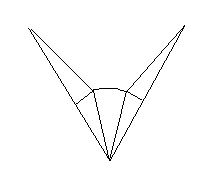
\includegraphics{PS/diag43.ps}
  \caption{The set measured by the function $K(S)$.}
  \label{fig:KS}
\end{figure}

In the remaining cases, each enclosed vertex has at least two
anchors.  Each anchor is a corner of the quad cluster.  Fix an
enclosed vertex $v$. Suppose that $v_1$, a corner, is an anchor of
$v$. Assume that the face $\{0,v,v_1\}$ bounds at most one upright
quarter. We sweep around the edge $\{0,v_1\}$, away from the
upright quarter if there is one,  until we come to another
enclosed vertex $v'$ such that $\{0,v_1,v'\}$ has circumradius
less than $\sqr2$ or such that $v_1$ is an anchor of $\{0,v'\}$.
If such a vertex $v'$ does not exist, we sweep all the way to
$v_2$ a corner of the quad cluster adjacent to $v_1$.

If $v'$ exists, then various
calculations\footnote{\calc{104677697}, \calc{69785808},
\calc{586706757}, and \calc{87690094}} give the bound
$-1.04\,\pt$, depending on the size of the circumradius of
$\{0,v,v'\}$. This allows us to assume that we do not encounter
such an enclosed vertex $v'$ whenever we sweep away, as above,
from the face formed by an anchor.

Now consider the simplex $S=\{0,v_1,v_2,v\}$, where $v_1$ is an
anchor of $\{0,v\}$.  We assume that it is not an upright quarter.
There are three alternatives. The first is that $S$ decreases the
score of the quarter by at least $0.52\,\pt$.
Calculations\footnote{\calc{185703487} and \calc{441195992}} show
that this occurs if the circumradius of the face $\{0,v,v_2\}$ is
less than $\sqr2$, or if the circumradius of the face is greater
than $\sqr2$, provided that the length of $\{v,v_1\}$ is at most
$2.2$. The second alternative\footnote{\calc{848147403},
\calc{969320489}, and \calc{975496332}.} is that the face
$\{0,v,v_1\}$ of $S$ is shared with a quarter $Q$ and that $S$ and
$Q$ taken together bring the score down by $0.52\,\pt$. In fact,
if there are two such simplices $S$ and $S'$ along $Q$, then the
three simplices $Q$, $S$, and $S'$ pull the
score\footnote{\calc{766771911}} below $-1.04\,\pt$. The third
alternative is that there is a simplex $S'=\{0,v,v,v_3\}$ sharing
the face $\{0,v,v_1\}$, which, like $S$, scores less than
$-0.31\,\pt$.  In each case, $S$ and the adjacent simplex through
$\{0,v,v_1\}$ score less than $-0.52\,\pt$. Since $v$ has at least
two anchors, the quad cluster scores less than $2(-0.52)\,\pt
=-1.04\,\pt$.
%
\end{proof}

\section{A Volume Formula}

In Definition~\ref{def:delta-e}, we found a solid $\delta(v,W ^e)$
that lies outside the ball of radius $t_0$ at $0$ but inside
$\op{VC}(0)$.  We now develop a formula for its volume.

Set $\phi_0=\phi(t_0,t_0)\approx -0.5666$. We define
    \begin{equation}\cro(h) =
2\pi(1-h/\eta_0(h))(\phi(h,\eta_0(h))-\phi_0). \end{equation} It
is equal to $-4\doct$ times the volume of the region outside the
sphere of radius $t_0$ and inside the finite cone
$C(h,\eta_0(h))$.  If $v$ is an enclosed vertex of height
$2h\in[2t_0,\sqr8$],
 such that every other vertex $v'$ of the
standard cluster satisfies
$$\eta(|v|,|v'|,|v-v'|)\ge \eta_0(h),$$ then the
solid represented by $\cro(|v|/2)$ lies outside the truncated
$V$-cell, but inside the $V$-cell, so that if $P$ is a quad
cluster,
 $$\op{c-vor}(V_P) < \op{c-vor}_0(V_P) + \cro(|v|/2).$$
If a vertex $v'$ satisfies $\eta(|v|,|v'|,|v-v'|)\le\eta_0(h)$,
then by the monotonicity of the circumradius of acute triangles,
$v'$ is an anchor of $v$.  This anchor clips the crown just
defined, and we add a correction term $\anc(|v'|,|v|,|v-v'|)$ to
account for this. Figure~\ref{fig:anchor} illustrates the terms in
the definition of $\anc()$.

\begin{figure}[htb]
  \centering
  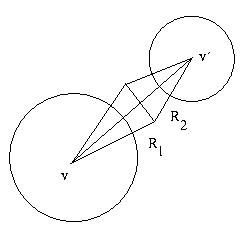
\includegraphics{PS/diag44.ps}
  \caption{An illustration of the terms $\anc$.}
  \label{fig:anchor}
\end{figure}


Set
    \begin{equation}
    \begin{array}{lll}
    \anc(y_1,y_2,y_6) &= -\dih(R_1)\cro(y_1/2)/(2\pi)
        -\sol(R_1)\phi_0+\op{r-vor}(R_1)\\
    &-\dih(R_2)(1-y_2/2t_0)(\phi(y_2/2,t_0)-\phi_0)
        -\sol(R_2)\phi_0 + \op{r-vor}(R_2),
    \label{eqn:4.5}
    \end{array}
    \end{equation}\index{anc@$\anc$}
where $R_i=R(y_i/2,\eta(y_1,y_2,y_6),\eta_0(y_1/2))$, for $i=1,2$.
In general, there are Rogers simplices on both sides of the face
$\{0,v,v')$, and this gives a factor of 2. For example, if $v$ has
a single anchor $v'$, then
$$\op{c-vor}(V_P) < \op{c-vor}_0(V_P) + \cro(|v|/2) + 2\anc(|v|,|v'|,|v-v'|).$$
However, if the anchor gives a face of an upright quarter, only
one side of the face lies in the $V$-cell,
 so that the factor of 2 is not required.
For example, $v'$ has context $\x(2,1)$ with upright quarter $Q$,
and if there are no other enclosed vertices, and if $v',v''$ are
the anchors along the faces of the quarter,  then
    $$
    \begin{array}{lll}
    \op{c-vor}(V_P)&< \op{c-vor}_0(V_P) +(1-\dih(Q)/(2\pi))\cro(|v|/2)\\
    &+\anc(|v|,|v'|,|v-v'|)+\anc(|v|,|v''|,|v-v''|).
    \end{array}
    $$
In general, when there are multiple anchors around the same
enclosed vertex $v$, we add a term $(2-k)\anc$ for each anchor,
where $k\in\{0,1,2\}$ is the number of quarters bounded by the
face formed by the anchor. We must be cautious (see
Condition~\ref{enum:wedge2} in Definition~\ref{def:wedge} in the
use of this formula. If the circumradius of $\{0,v,v',v''\}$ is
less than $\eta_0(|v|/2)$, the Rogers simplices used to define the
terms $\anc()$ at $v'$ and $v''$ overlap. When this occurs, the
geometric decomposition on which the correction terms $\anc()$ are
based is no longer valid. In this case, other methods must be
used.

\begin{figure}[htb]
  \centering
  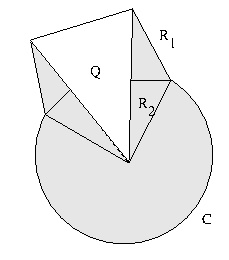
\includegraphics{PS/diag46.ps}
  \caption{The terms $\anc$ near an upright quarter.}
  \label{fig:anchor-quarter:bis}
\end{figure}

\smallskip
If $(P,D)$ is a mixed quad cluster, let $(P,D')$ be the new quad
cluster obtained by removing all the enclosed vertices.  We define
a $V$-cell $V(P,D')$ of $(P,D')$ and the truncation of $V(P,D')$
at $t_0$. We take its score $\op{vor}_{0,P}(D')$  as we do for
standard clusters.  $(P,D')$ does not contain any quarters.

\begin{lemma} \label{lemma:mixed-vor0}
%\proclaim{Proposition 4.7}
If $(P,D)$ is a mixed quad cluster, $\sigma_P(D') <
\vor_{0,P}(D)$.
\end{lemma}

\begin{remark}
The special case of the proof where an upright quarter has context
$c(Q)=(2,1)$ will be applied in Section~\ref{x-3.3} in situations
other than mixed quad clusters.
\end{remark}

\begin{proof}
%
Suppose there exists an enclosed vertex that has context
$\x(2,1)$; that is, there is a single upright quarter
$Q=S(y_1,y_2,\ldots,y_6)$ and no additional anchors.  In this
context $\sigma(Q)=\mu(Q)$. Let $v$ be the enclosed vertex.  To
compare $\sigma_P(D)$ with $\vor_{0,P}(D')$, consider the $V$-cell
near $Q$. The quarter $Q$ cuts a wedge of angle $\dih(Q)$ from the
crown at $v$. There is an anchor term for the two anchors of $v$
along the faces of $Q$. Let $V_P^v$ be the truncation at height
$t_0$ of $V_P$ near $v$ and under the four Rogers simplices
stemming from the two anchors.
(Figure~\ref{fig:anchor-quarter:bis} shades the truncated parts of
the quad cluster.) As a consequence
\smallskip
    \begin{equation}
        \op{c-vor}(V_P) <(1-\dih(Q)/(2\pi))\cro(y_1/2)+\anc(y_1,y_2,y_6)
        +\anc(y_1,y_3,y_5) +\op{c-vor}(V_P^v).
    \label{eqn:4.8}
    \end{equation}
Combining this inequality with
calculations\footnote{\calc{906566422}, \calc{703457064}, and
\calc{175514843}}, we find
    \begin{equation}
        \op{c-vor}(V_P) +\mu(Q) < \op{c-vor}(V_P^v) +\svor_0(Q).
        \label{eqn:4.9}
    \end{equation}

Now suppose there is an enclosed vertex $v$ with context
$\x(3,1)$. Let the quad cluster have corners $v_1$, $v_2$, $v_3$,
$v_4$, ordered consecutively.  Suppose the two quarters along $v$
are $Q_1=\{0,v,v_1,v_2\}$ and $Q_2=\{0,v,v_2,v_3\}$.  We consider
two cases.

\noindent Case 1:  $\dih(Q_1)+\dih(Q_2)<\pi$ or
$\rad(0,v,v_1,v_3)\ge\eta(|v|,2,2t_0)$. In this case, the use of
correction terms to the crown are legitimate as in
Definition~\ref{def:wedge}. Proceeding as in context $\x(2,1)$, we
find that
\smallskip
    \begin{equation}
    \op{c-vor}(V_P) < (1-(\dih(Q_1)+\dih(Q_2))/(2\pi))\cro(|v|/2)
    +\anc(F_1) +\anc(F_2) +\op{c-vor}(V_P^v).
    \label{eqn:4.10}
    \end{equation}
Here $V_P^v$ is defined by the truncation at height $t_0$
 under the $V$-face determined by $v$ and
under the Rogers simplices stemming from the side of $F_i$ that
occur in the definition of $\anc$. Also,
$\anc(F_i)=\anc(y_i,y_j,y_k)$ for a face $F_i$ with edges $y_i$
along an upright quarter. By a
calculation\footnote{\calc{554253147}} applied to both $Q_1$ and
$Q_2$, we have
    \begin{equation}
    \op{c-vor}(V_P) +\sum_{i=1}^2\sigma(Q_i)
    < \op{c-vor}(V_P^v) + \sum_{i=1}^2 \svor_0(Q_i).
    \label{eqn:4.11}
    \end{equation}
That is, by truncating near $v$, and changing the scoring of the
quarters to $\svor_0$, we obtain an upper bound on the score.

\noindent Case 2:  $\dih(Q_1)+\dih(Q_2)\ge\pi$ and
    $\rad(0,v,v_1,v_3)\le \eta_0(|v|/2)$.
The anchor terms cannot be used here. In the mixed case,
$\sqr8<|v_1-v_3|$, so
$$\sqr2<{\frac{1}{2}}|v_1-v_3|\le\rad \le \eta_0(|v|/2),$$
and this implies $|v|\ge 2.696$. We
have\footnote{\calc{855677395}}
$$\sum_{i=1}^2 \sigma(Q_i) < \sum_{i=1}^2 \svor_0(Q_i) +
\sum_{i=1}^2 0.01(\pi/2-\dih(Q_i))< \sum_{i=1}^2 \svor_0(Q_i).$$
Inequality~\ref{eqn:4.11} holds, for $V_P^v=V_P$.

In the general case, we run over all enclosed vertices $v$ and
truncate around each vertex.  For each vertex we obtain
Inequality~\ref{eqn:4.9} or \ref{eqn:4.11}. These inequalities can
be coherently combined over multiple enclosed vertices because the
$V$-faces were associated with different vertices $v$ and none of
the Rogers simplices used in the terms $\anc()$ overlap. More
precisely, if $Z$ is a set of enclosed vertices, set $V_P^Z =
\cap_{v\in Z} V_P^v$, and $V_P^{v,Z} = V_P^Z\cap V_P^v$. Coherence
means that we obtain valid inequalities by adding the superscript
$Z$ to $V_P$ and $V_P^v$ in Inequalities~\ref{eqn:4.9} and
\ref{eqn:4.11}, if $v\not\in Z$. In sum,
    $\sigma_P(D) < \vor_{0,P}(D)$.
%
\end{proof}
